\chapter{Aktører}\label{Aktorer}

Aktørerne kan enten påvirke eller blive påvirket af systemet. Primære aktører er interessenter, der kalder på systemet til at levere service, mens sekundære aktører leverer en service til systemet. 

Tabel \ref{Beskriv} viser aktørbeskrivelser, og hvordan hver aktør interagerer med Automatisk Ultralydsscanner. 

\section{Aktørbeskrivelse}
\begin{table}[htb]
\begin{tabular}{|l|l|p{0.6\textwidth}| }
  \hline
  \textbf{Aktørnavn} & \textbf{Type} & \textbf{Beskrivelse} \\ \hline
  Operatør & Primær & Operatør betjener Automatisk Ultralydsscanner 
  \\ \hline
  Patient & Sekundær & Patient er personen, hvorpå scanningen foregår \\ \hline
  Robotarm & Sekundær & Robotarm styrer Ultralydsscanner i det detekterede brystområde \\ \hline
Ultralydsscanner & Sekundær & Ultralydsscanner danner ultralydsvideoclips, som Operatør kan følge på Ultralydsscanners skærm\\ \hline
  3D kamera & Sekundær & 3D kamera scanner det brystområde, hvorpå Ultralydsscanner skal foretage scanning \\ \hline 
\end{tabular}
\caption{Aktørbeskrivelse}
\label{Beskriv}
\end{table}
\newpage

\subsection{Aktør-kontekst diagram}
I figur \ref{akDiagram} ses et aktør-kontekst diagram, som viser interaktionen mellem aktørerne og PC Applikation. Primære aktører er afbilledet på venstre side og de sekundære er afbilledet på højre side.

\begin{figure}[H]
    \centering
    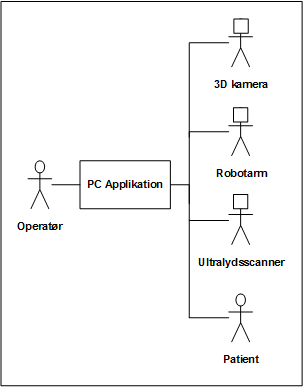
\includegraphics[width=0.70\textwidth]{figurer/d/Kravspecifikation/uml_aktor}
    \caption{Aktør-kontekstdiagram.}
    \label{akDiagram}
\end{figure}